
%%%%%%%%%%%%%%%%%%%%%%%%%%%%%%%%%%%%%%%%%%%%%%%%%%%%%%%%%%%%%%%%%%%%%%%%%%%%%%%%
%% CAPITULO
%%%%%%%%%%%%%%%%%%%%%%%%%%%%%%%%%%%%%%%%%%%%%%%%%%%%%%%%%%%%%%%%%%%%%%%%%%%%%%%%
\chapterimage{chapter_head_2.pdf} % Chapter heading image

\chapter{\textcolor{blue}{Passos do samba de gafieira}}
%\index{Passos}

\begin{definition}[Plano axial:] 
\index{Plano axial}
\label{def:PlanoAxial}
O Dicionário Priberam da Língua Portuguesa \cite{priberamplano} define plano axial como:
Plano transversal, plano horizontal que divide o corpo ou uma estrutura anatômica em parte superior e parte inferior.
Ver Figura \ref{fig:bodyhumanplane}.
\end{definition}

\begin{definition}[Plano frontal:] 
\index{Plano frontal}
\label{def:PlanoFrontal}
O Dicionário Priberam da Língua Portuguesa \cite{priberamplano} define plano frontal como:
Plano coronal,   plano vertical e paralelo à sutura coronal do crânio, que divide o corpo em parte anterior e parte posterior.
Ver Figura \ref{fig:bodyhumanplane}.
\end{definition}

\begin{definition}[Plano sagital:] 
\index{Plano sagital}
\label{def:PlanoSagital}
O Dicionário Priberam da Língua Portuguesa \cite{priberamplano} define plano sagital como:
Plano vertical e paralelo à sutura sagital do crânio, que divide o corpo em parte direita e parte esquerda.
Ver Figura \ref{fig:bodyhumanplane}.
\end{definition}

\begin{figure}[h]
  \centering
    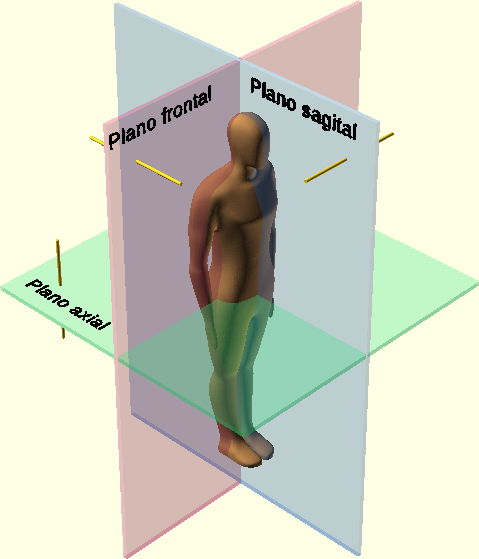
\includegraphics[width=0.40\textwidth]{body-plane/files/body-plane.png}
  \caption{ Planos e eixos no corpo humano.}
\label{fig:bodyhumanplane}
\end{figure}

\begin{definition}[Eixo axial:] 
\index{Eixo axial}
\label{def:EixoAxial}
É o eixo perpendicular ao plano axial.
Ver Figura \ref{fig:bodyhumanplane}.
\end{definition}

\begin{definition}[Eixo frontal:] 
\index{Eixo frontal}
\label{def:EixoFrontal}
É o eixo perpendicular ao plano frontal.
Ver Figura \ref{fig:bodyhumanplane}.
\end{definition}

\begin{definition}[Eixo sagital:] 
\index{Eixo sagital}
\label{def:EixoSagital}
É o eixo perpendicular ao plano sagital.
Ver Figura \ref{fig:bodyhumanplane}.
\end{definition}

\begin{definition}[Passo cíclico:] 
\index{Passo cíclico}
\label{def:PassoCiclico}
É um passo de dança que pode acontecer por um tempo indeterminado,
devido a que este está composto por ciclos, cuja postura de inicio e final é a mesma.
\end{definition}

\begin{definition}[Duração do passo:] 
\index{Duração do passo}
\label{def:DuracaoDoPasso}
É a longitude temporal de um passo de dança, contado em tempos da música.
No caso de \hyperref[def:PassoCiclico]{\textbf{passos cíclicos}}, a duração do passo se refere a duração do ciclo.
\end{definition}


\begin{definition}[Dançar em tempo:] 
\index{Dançar no tempo}
\label{def:DancaNoTempo}
É um passo de dança onde o movimento principal ou inicial, dependendo do estilo de dança, 
se executa no tempo forte da música.
\end{definition}

\begin{definition}[Dançar em contratempo:] 
\index{Dançar no contratempo}
\label{def:DancaNoContratempo}
É um passo de dança onde o movimento principal ou inicial, dependendo do estilo de dança, 
se executa em contra do tempo forte da música; é dizer, em contratempo.
\end{definition}

\begin{definition}[Passo a contratempo:] 
\index{Passo a contratempo}
\label{def:PassoAContratempo}
É um passo de dança cuja execução promove que quando se esteja dançando com um pé especifico acompanhando o tempo forte da música,
ao finalizar o passo este pé esteja sendo marcado no tempo fraco.
É dizer, são movimento onde após de realizados, passamos de \hyperref[def:DancaNoTempo]{\textbf{dançar no tempo}} a \hyperref[def:DancaNoContratempo]{\textbf{dançar no contratempo}} e vice-versa. 
\end{definition}



%%%%%%%%%%%%%%%%%%%%%%%%%%%%%%%%%%%%%%%%%%%%%%%%%%%%%%%%%%%%%%%%%%%%%%%%%%%%%%%
\section{\textcolor{blue}{Quais são os passos de samba de gafieira?}}

Existem na atualidade uma grande variedade de passos para o samba de gafieira,
tantos como a imaginação possa atingir, pois além dos movimentos mais conhecidos e  consagrados da dança,
podem existir variações  destes ou simplesmente estilos em que estos são realizados. 

Nos seguintes parágrafos desta seção, listaremos e descreveremos 
alguns dos passos que são possíveis de ver no samba de gafieira;
mas, estas descrições não pretendem ser uma guia de ensino,
e sim um instrumento para saciar a curiosidade do leitor em como os movimentos são realizados.\\

Nos passos que eram possíveis de ver do samba de gafieira (primigênio) temos \cite[pp. 142]{perna2002samba}:
\begin{itemize}
\item \textbf{Balão}, 
\index{Passo!Balão}
este movimento pode ser considerado aéreo, 
pois o \hyperref[def:Condutor]{\textbf{condutor}} tira do chão os pés do \hyperref[def:Seguidor]{\textbf{seguidor}}.
O movimento dura 3 tempos, o passo inicia com o seguidor ao lado direito do condutor, 
ligeiramente atrás dele, com um abraço de dança bem próximo.
No primeiro tempo o condutor da um passo ao lado, e pisa com o pé direito,
de modo que o seguidor fique em pé atrás da perna dele, sem perder o abraço.
No segundo tempo, aproveitando a postura, 
o condutor faz um movimento circular anti-horário com seu quadril, no \hyperref[def:PlanoAxial]{\textbf{plano axial}},
de modo que sua perna direita, que está em contato com a perna direita do seguidor,
serva como alavanca para tirar ao seguidor do chão, 
e este gire ou voe ao redor \footnote{O giro do seguidor é com o corpo reto e pernas juntas, 
como se fosse uma fita solta de um lado e com um lado presso num eixo que provoca a esta girar no \hyperref[def:PlanoAxial]{\textbf{plano axial}} do eixo de giro.} 
do condutor em sentido anti-horário.
No terceiro tempo o seguidor senta-se, é dizer faz uma cadeirinha, sobre a perna esquerda do condutor,
que para receber ao seguidor da um passo ao frente. 

\item \textbf{Balão apagado},
\index{Passo!Balão apagado} este movimento tem um parecido ou lembrança com o \textbf{Balão}; 
porem, o \hyperref[def:Seguidor]{\textbf{seguidor}} não voa ao redor do \hyperref[def:Condutor]{\textbf{condutor}}, 
se não que a intenção de voar se apaga e o seguidor nunca sai do chão; 
de modo que o casal fica dando giros, abraçados, num eixo comum e praticamente no lugar. 
Estes giros são promovidos por marcados movimentos circulares de quadril, que mudam
de velocidade e intenção num constante, abrupto, leve e leve,  na proporção de tempos \{1/2 tempo,1/2 tempo, tempo\}; 
semelhando assim ao movimento de um balão perdendo o ar.
Existem variantes deste movimento, onde o giro do par é realizado em sentido horário e anti-horário; porem, 
não saberia afirmar qual é a versão original, mas pelas minhas observações a versão mais difundida,
é a que faz o giro  anti-horário.

Este passo é um movimento cíclico, com ciclos que duram 4 tempos, 
sendo o primeiro par de tempos similar ao segundo, porem com os papeis intercambiados no par de dança.
No momento inicial, o casal está abraçado numa postura frente a frente, 
com o peso do corpo do lado da perna direita do condutor;
no tempo 1 o condutor da um passo e pisa com a perna esquerda pra traz, 
como se procura-se ocultar esta atrás da sua perna direita, 
este movimento de perna é promovido pelo movimento circular do quadril em sentido anti-horário no \hyperref[def:PlanoAxial]{\textbf{plano axial}};
por outro lado, 
o seguidor da um passo adiante com sua perna direita procurando manter a postura relativa com o condutor e acompanhando o movimento circular anti-horário do quadril, 
de modo que se seu pé direito tende a procurar rodear ao condutor.
Nos tempos 1.5 e 2 o par pisa no lugar, ajeitando suas posturas apagando o movimento do quadril, 
mas mantendo o giro do par, 
de modo que terminam abraçados  frente a frente com o peso do corpo no lado do pé esquerdo do condutor.
No próximo par de tempos, o movimento é similar, só que agora é o seguidor que inicia dando um passo com o pé esquerdo. 

\item \textbf{Pica-pau} \index{Passo!Pica-pau}. 
\end{itemize}~\\



Os movimentos que já existiam antes de 1986 são \cite[pp. 6]{gafieiraaredeout2}:
\begin{itemize}
\item \textbf{Cadeirinha} 
\index{Passo!Cadeirinha}
Pode ser vista uma fotografia da posse final, caraterística deste movimento, no ``jornal dos sports''(RJ),
do dia 17 de julho de 1986 \cite[pp. 6]{gafieiraaredeout2}.

\item \textbf{Puladinho}, 
\index{Passo!Puladinho} 
neste movimento não se pula; 
existem varias referencias não acadêmicas na internet, que datam desde o 2002,
onde não mencionam ao ``Puladinho'' e sim um passo chamado ``pruladinho'', 
pelo qual suspeito que este faz referencia ao mesmo passo;
pois indica corretamente que no movimento se vá ``pra o ladinho''.

Podemos achar uma referencia ao uso do termo puladinho numa música instrumental chamada 
``Puladinho na gafieira'' (1958)  de  Marisa com Moacyr Silva e seu conjunto: Convite à música \cite{puladinhogafieiramusic}.

Finalmente, podemos ver uma referencia a esse passo de dança, no ``jornal dos sports''(RJ),
do dia 17 de julho de 1986 \cite[pp. 6]{gafieiraaredeout2}.
\end{itemize}~\\

Em palavras de Jimmy de Oliveira os movimentos que já existiam antes do 1990 são \cite{sambafunkeadoJimmyDeOliveiraPart1}:
\begin{itemize}
\item \textbf{Picadilho}
\index{Passo!Picadilho}
ou picadinho, é um movimento de pouco deslocamento, 
se realiza com um abraço mais folgado, 
para dar espaço ao movimento do \hyperref[def:Seguidor]{\textbf{seguidor}}, ou a entidade feminina do par.
Cada ciclo do movimente dura 4 tempos, sendo o primeiro par de tempos do passo, simétrico ao segundo.
Para uma correta execução do movimento, o condutor envia informação de condução mediante o abraço de dança,
de modo que esta informação chegue quase sem degradação ate o quadril do seguidor,
é nesse ponto que a condução provoca o movimento das pernas (uma por vez), de modo que
o seguidor mantêm em todo momento as ``pernas fechadas''\footnote{
Ter as pernas fechadas, neste contexto, não indica literalmente ter as pernas juntas, 
e sim juntar as pernas como se em todo momento ao caminhar tentássemos segurar uma folha de papel na virilha.}.
Assim, na primeira metade do ciclo do passo, o seguidor,
da inicialmente um passo ao frente ganhando o peso do corpo (e descansa médio tempo), 
logo o pé livre que está atrás faz um movimento para fechar mais as pernas (e descansa médio tempo), 
ganhando este pé o peso do corpo, logo o novo pé livre se movimenta ligeiramente ao frente, 
para ajeitar a postura e ganhar o peso do corpo (e descansa um tempo).
A segunda metade do ciclo é similar à primeira só que agora se inicia com o outro pé, 
o pé livre do peso do corpo.

\item \textbf{Pião}, 
\index{Passo!Pião}
este movimento é executado, com o casal abraçado, realizando giros sobre um eixo comum.
Cada giro ou ciclo dura tradicionalmente 2 tempos, e é realizado em sentido horário;
na primeira metade do ciclo (que dura 1 tempo) o eixo de giro do par é colocado sobre uma pessoa do par, 
de modo que a outra pessoa gira ao redor (em 1 tempo), ate chegar a uma postura similar à inicial, 
porem com as posturas intercambiadas no par;
na outra metade do ciclo se repete o movimento, porem agora é a outra pessoa que terá o eixo do par.
Este é um movimento de deslocamento, de modo que se procura girar movimentando-se numa linha reta.
\end{itemize}~\\

Os passos criados a finais da década de 1980 e inícios de 1990 são \cite[pp. 143]{perna2002samba}:
\begin{tasks}
\task \textbf{Caminhada}, \index{Passo!Caminhada a contratempo}ou caminhada a contratempo.
\task \textbf{Chicote} \index{Passo!Chicote}.
\task \textbf{Esse} \index{Passo!Esse}.
\task \textbf{Facão} \index{Passo!Facão}.
\task \textbf{Faquinha} \index{Passo!Faquinha}.
\task \textbf{Gancho} \index{Passo!Gancho}.
\task \textbf{Gancho redondo} \index{Passo!Gancho redondo}.
\task \textbf{Letra} \index{Passo!Letra}.
\task \textbf{Puladinho redondo} \index{Passo!Puladinho redondo}.
\task \textbf{Trança} \index{Passo!Trança}.
\task \textbf{Tesoura} \index{Passo!Tesoura}.
\end{tasks}~\\


Os passos criados por Jimmy de Oliveira, apos o ano 1990 são \cite{sambafunkeadoJimmyDeOliveiraPart1}: 
\begin{tasks}
\task \textbf{Assalto} \index{Passo!Assalto}. 
\task \textbf{Boneca} \index{Passo!Boneca}.
\task \textbf{Elástico} \index{Passo!Elastico}.
\task \textbf{Escovinha} \index{Passo!Escovinha}.
%\task \textbf{Homem na lua}.  
\task \textbf{Pescaria} \index{Passo!Pescaria}.
\task \textbf{Romário} \index{Passo!Romário}.
\end{tasks}~\\


Outros movimentos sem data conhecida são \cite[pp. 143]{perna2002samba}:
\begin{tasks}
\task \textbf{Bicicleta} \index{Passo!Bicicleta}.
\task \textbf{Cruzado} \index{Passo!Cruzado}.
\end{tasks}~\\


Passos acrobáticos ou para apresentações \cite[pp. 142-143]{perna2002samba}:
\begin{tasks}
\task \textbf{Cabide}, \index{Passo!Cabide} oriundo do rock.
\task \textbf{Baratinha} \index{Passo!Baratinha}
\task \textbf{Enceradeira}, \index{Passo!Enceradeira} criado em algum momento no final da década de 1980 e inícios da década de 1990.
\end{tasks}


%%%%%%%%%%%%%%%%%%%%%%%%%%%%%%%%%%%%%%%%%%%%%%%%%%%%%%%%%%%%%%%%%%%%%%%%%%%%%%%
\section{Sobre o $syllabus$ da samba de gafieira}

O $syllabus$  do samba de gafieira, foi criado no ano 2001 em Rio de Janeiro,
este é um listado de passos ordenado em três níveis (básico, intermediário e avançado),
selecionados por votação,
onde são agrupados passos que se consideram essenciais para o ensino e competição;
neste listado não entram passos aéreos \cite[pp. 144]{perna2002samba}.


As personas que participaram da votação para a elaboração do $syllabus$ são \cite[pp. 144]{perna2002samba}:
\begin{inparaitem}[$*$]
\item Bob Cunha e Aurya
\item Bolacha
\item Bruno Barros
\item Carlinhos de Jesus
\item Dani Aguiar
\item Dani Escudero
\item Dani Galper
\item Egídio
\item Flávio Miguel
\item Gérson Reis
\item Kilve
\item Luis Florião/Adriana
\item Marcello Moragas
\item Marco Antonio Perna
\item Marquinhos Copacabana
\item Rogério Mendonça
\item Valdeci
\item Wanir Almeida
\end{inparaitem}.\\



Os passos de \textbf{nível básico} são:
\begin{tasks}(2)
\task Básico (frente-trás)
\task Balanço 
\task Caminhada (ou caminhada a contratempo)
\task Cruzado
\task Esse
\task Gancho
\task Giro da dama
\task Puladinho
\task Saída lateral
\task Tirada ao lado
\end{tasks}~\\


Os passos de \textbf{nível intermediário} são:
\begin{tasks}(2)
\task Assalto
\task Balão apagado
\task Escovinha
\task Facão
\task Gancho redondo
\task Mestre sala
\task Romário
\task Tesoura
\task Tirada de perna
\task Trança
\end{tasks}~\\

Os passos de \textbf{nível avançado} são:
\begin{tasks}(2)
\task Bicicleta
\task Enceradeira
\task Pião
\task Picadinho (ou ou picadilho)
\task Pica-pau
\end{tasks}

